\vspace*{1.5pc}

%%%%%%%%%%%%%%%%%%%%%%%%%%%%%%%%%%%
\subsection{Quasars and their Absorption Features}
%%%%%%%%%%%%%%%%%%%%%%%%%%%%%%%%%%%

\subsubsection{Quasi Stellar Objects}
\label{sec:qso}

Quasi Stellar Objects (QSO) \textit{a.k.a.} quasars are believed to be powered by the accretion of matter onto Supermassive Black
Holes (SMBH) at the center of galaxies. The accression process is a very efficient energy conversion mechanism, as its ratio is of the order of the compacity of the central compact object. As such, quasars are the brightest objects in the Universe, as they can emit more energy than any other known process, chemical or thermonuclear, including supernov{\ae}. They are considered to be the most luminous members of a more general class of objects called Active Galactic Nuclei (AGNs). Quasars appear point or star-like in optical images but spectroscopic observations reveal they are widely different objects in several ways. Their intrinsic luminosities can reach as high as $10^{14}~L_\odot$ solar luminosities, but can vary in brightness at different wavelengths on timescales as short as days or weeks. \\

Their small size along with these orders of luminosities led to consider gravity as their energy source immediately upon their discovery in the 1960's~\citep{Matthews1963}. The required gravitational potential energy can be extracted if quasars contain compact objects with masses of $\sim 10^{8-9}~ M_\odot$ solar masses and sizes about that of the solar system. The
gravitational field of such objects is so strong that the effects of general relativity are dominant in their vicinity. There have been many proposed candidates for such a source of energy. Nowadays, it is believed that quasars and AGNs are powered by SMBH of billions of solar masses. The radiated energy we detect from them comes from matter being accreted onto the black hole. The radii of black holes in AGNs and quasars range from a few solar radii to 20 astronomical units. The matter surrounding the central black hole is likely to form an accretion disk, in which some source of viscosity drains the orbiting matter from angular momentum, making it spiral inwards toward the central black hole. The gas in the inner
regions of the disk is expected to be as hot as $10^{4-6}~\mathrm{K}$, hot enough to account for the thermal component of the continuum radiation at  ultraviolet wavelengths. \\

One of the most distinctive features of quasars is their large redshifts. The Baryon Oscillations Sky Survey (introduced later in Sec.~\ref{sec:pfdata}) has detected $\sim 45$ quasars with a redshift greater than 5 \citep{Paris2013}, the farthest detected QSO being being at $z=7.085$
\citep{Mortlock2011}. However, most known quasars have redshifts lesser than $z \leq 2.5$, in part because they are easier to find but also because they are intrinsically more numerous, as quantified by the QSO luminosity function ~\citep{Palanque-Delabrouille2013a}. The lower redshift limit for quasars is arbitraily set at $z \geq 0.1$ since they become resolvable as galaxies and usually catalogued as AGNs. In addition to providing our first view of the Universe beyond redshifts $z \geq 5$, quasars are also valuable cosmological probe. Indeed, they are luminous enough to trace the matter distribution at those very distant scales and very old lookback times. They also entail properties of the matter distribution along the line-of-sight.

\begin{figure}
\begin{center}
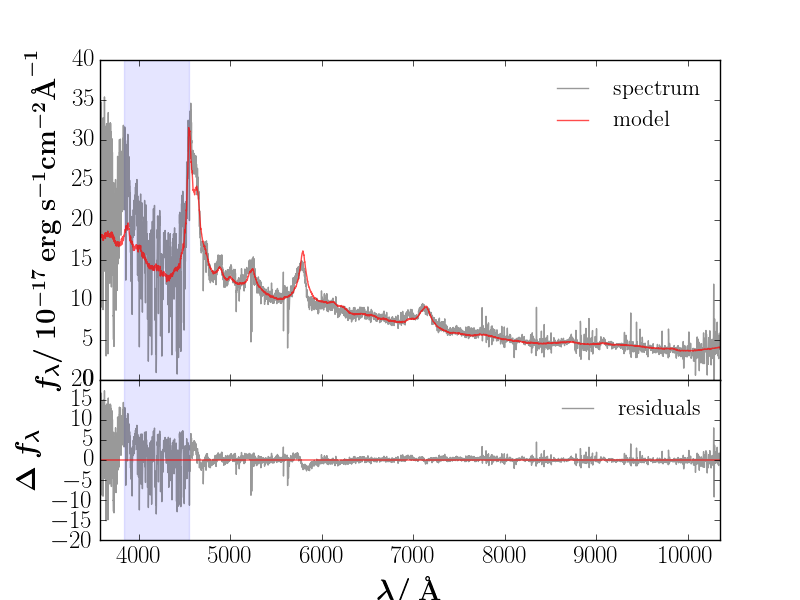
\includegraphics[width=0.8\columnwidth]{BOSS_spectrum.png}
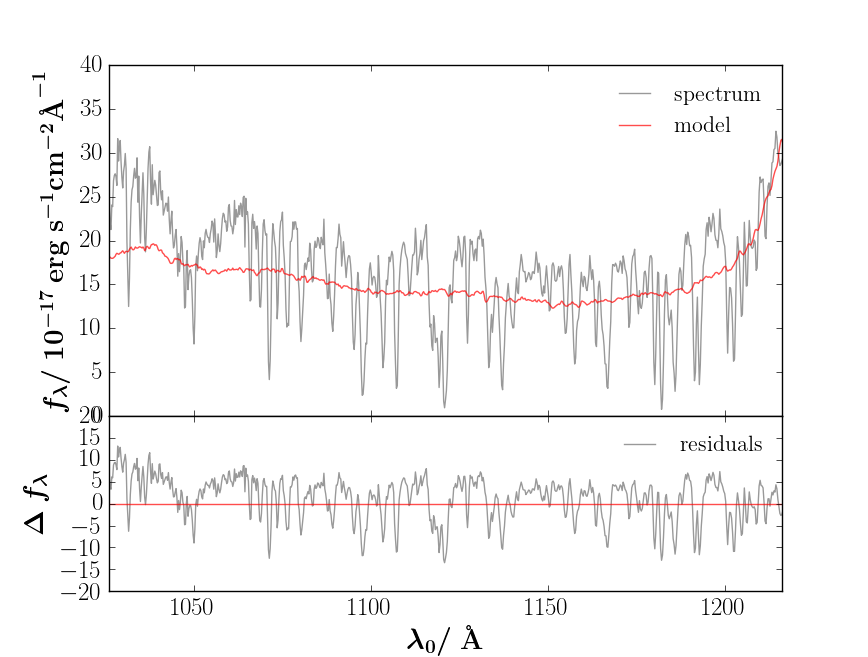
\includegraphics[width=0.8\columnwidth]{BOSS_Lya.png}
\caption{\textbf{Top:} Optical spectrum of a generic quasar in the BOSS data set in the observed wavelength $\lambda_0$. The red line is a spectrum model fitted in the data reduction pipeline, the residuals being in the lower panel. The region highlighted in blue is the Ly-$\alpha$ forest wavelength range. \textbf{Bottom:} Zoom in on the Ly-$\alpha$ forest range highlighted in blue in the top panel.}
\label{fig:boss_spectrum}
\end{center}
\end{figure}

\subsubsection{Emission Lines}

Quasars emit from gamma and X rays to the hundred-micron far infrared (FIR) wavelengths. The energy emitted in each band is usually similar, in stark contrast to stars, whose thermal radiation peak and restrict the emission in wavelength. Most quasars at $z \leq 2.5$ are bright in ultraviolet (UV), a helpful property in distinguishing them from stars in sky surveys, which are more numerous and usually faint in UV. The continuum emission in quasars appears to arise from a combination of thermal and non-thermal processes. In any event, the continuum radiation from quasars demonstrates that some very energetic processes are involved. It can be modeled by a continuum that follows a power law in wavelength, on top of which there are a number of emission and absorption features. The width of an emission line is determined by the velocity dispersion of the gas in the emitting region, where a mixture of infall, rotation and ejection probably occurs. The widths
are consistent with the emission region being at a distance of light months to a few light-years from a central black hole. The strongest emission lines in quasar spectra come from Hydrogen, Carbon and Magnesium ions, with lines of Nitrogen, Oxygen, Iron and other metals also being visible. The observed levels of ionization range from neutral for Hydrogen and Oxygen to five
times ionized Oxygen and even more highly ionized Iron. Several absorption lines are visible in the spectra in the upper panel of Fig.~\ref{fig:boss_spectrum}.


\subsubsection{Absorption Lines}

Absorption lines were observed in quasars a few years after their initial discovery and were believed at the time to be quite rare. Nowadays, the
study of quasar absorption lines is a major topic in astrophysics. Depending on the distance of the absorbing gas from the central emission source of the quasar, absorption lines are said to either be caused by either \emph{intrinsic}, \emph{associated} or \emph{intervening} systems. \\

Intrinsic systems arise from either the accretion disk or the collimated jets that run perpandicular to the acretion disk's plane. An example of an intrinsic system are Broad Absorption Line (BAL) quasars, whose spectra show very wide absorption troughs blue-wards of the emission lines. The widths of these absorption features indicate outflow velocities that can exceed $3 \times 10^4~\mathrm{km}~s^{-1}$. Associated systems show absorption features from elements such as Hydrogen, Carbon and Magnesium which are narrower than the emission lines and slightly blue-shifted. This suggests they arise in the gas of the host galaxy of the quasar or its environment. Intervening systems on the other hand, can have significantly lower redshifts than the emission lines, suggesting they arise from the intergalactic gas exterior to the quasar that lies along the line-of-sight. In this case, the quasar acts as a background beacon and enables the study of that intermediary gas, which has provided crucial information about the gas in the early Universe, from its distribution to its thermodynamic properties. \\

Depending on the column density of the absorbing gas, intervening systems are themselves broken down into $3$ main categories: \\

\begin{enumerate}
	\item[$\bullet$] Damped Lyman-$\alpha$ Systems (DLA), with column densities in excess of $10^{20}$ neutral Hydrogen atoms per $\mathrm{cm}^2$. These manifest as saturations in the absorption, and occurs when the light travels through a galaxy for instance; \\
	\item[$\bullet$] Lyman limit or intermediate systems, with $N_{\textsc{Hi}} \sim 10^{16-20}~ \mathrm{cm}^{-2}$, commonly attributed to the gas present in galaxy halos; and \\
	\item[$\bullet$] the Lyman-$\alpha$ forest, with $N_{\textsc{Hi}} \sim 10^{12-14}~ \mathrm{cm}^{-2}$, attributed to the gas in the IGM. \\
\end{enumerate}

The Lyman-$\alpha$ forest absorption lines are the most numerous and ubiquitous absorption features in the spectra of quasars with intervening systems in the foreground. In Sec.~\ref{sec:def_lya}, I detail how the Ly-$\alpha$ forest can be used to garner insight on the intergalactic gas.


%%%%%%%%%%%%%%%%%%%%%%%%%%%%%%%%%%%
\subsection{Absorption in the IGM}
%%%%%%%%%%%%%%%%%%%%%%%%%%%%%%%%%%%

\subsubsection{Characteristics of Light}

The equation that governs the interactions between radiation and matter is the \textbf{transfer equation} \\
\begin{empheq}[box=\mymath]{equation}
\frac{\partial I_\nu}{\partial t} + \left( c \vec{k} \cdot \vec{\nabla} \right)~I_\nu = 0
\end{empheq} \\ which is a balance on the conserved quantity $I_\nu$, the specific intensity. It is defined such that the energy that propagates from point $M$ on surface $d\Sigma$ during a time interval $dt$ within solid angle $d\Omega$ of direction $\vec{k}$ at frequency $\nu \pm d\nu$ is
\begin{equation}
dE_\nu = I_\nu ~d\nu~ dt~ \mu~ d\Omega~ d\Sigma
\end{equation} with $\mu = \vec{k} \cdot \vec{n} = \cos \theta$. Characterising radiation \textit{a priori} requires the knowledge of 7 parameters: position ($x$, $y$, $z$), direction ($\theta$, $\varphi$), instant in time ($t$) and frequency ($\nu$). However, in general, not all these information are necessary. For far enough sources of light where their shape does not matter all that much, as is the case for distant quasars, the moments of the specific intensity are sufficient to fully characterise their radiation.  The zeroth, first and second moments of $I_\nu$ with respect to $\mu = \cos \theta$ are respectively the \textbf{spectral energy density}, the \textbf{flux} and the \textbf{spectral radiation pressure density}:\\

\begin{equation}
\label{sys:mominu}
\left\{
\begin{array}{ll}
u_\nu = \cfrac{2\pi}{c}~ \displaystyle \int_{-1}^{1} d\mu ~I_\nu & = \cfrac{4\pi}{c} J_\nu \\
\varphi_\nu = 2\pi~ \displaystyle \int_{-1}^{1} d\mu ~\mu ~I_\nu & = \pi ~ I_\nu \\
P_\nu = \cfrac{1}{c}~ \displaystyle \int_{-1}^{1} d\mu ~\mu^2 ~I_\nu & = \cfrac{u_\nu}{3}
\end{array}
\right.
\end{equation} \\ where the mean specific intensity is $\displaystyle \int d\Omega ~I_\nu = 4\pi~J_\nu$. The flux in Eq.~\ref{sys:mominu} is defined such that it is an implicit function of frequency. A common unit in which the flux of high redshift galaxies and quasars is expressed in is the Jansky where $1 ~\mathrm{Jy} = 10^{-26} W m^{-2} \mathrm{Hz}^{-1}$. The net (bolometric) flux of a light source is simply $\varphi = \displaystyle \int_0^\infty d\nu~\varphi_\nu$. The flux diminishes with distance from the source, following an inverse square law. The specific intensity, however, is constant along a light ray unless there is absorption, emission or scattering of the photons along the way. When that is the case, the transfer equation must include source, drain and exchange terms. In this thesis work, I consider quasars, which I've introduced in Sec.~\ref{sec:qso}, as a background source and the neutral Hydrogen in the forground as an absorber.

\subsubsection{Optical Depth}
\label{sec:optdep}

\begin{figure}
\begin{center}
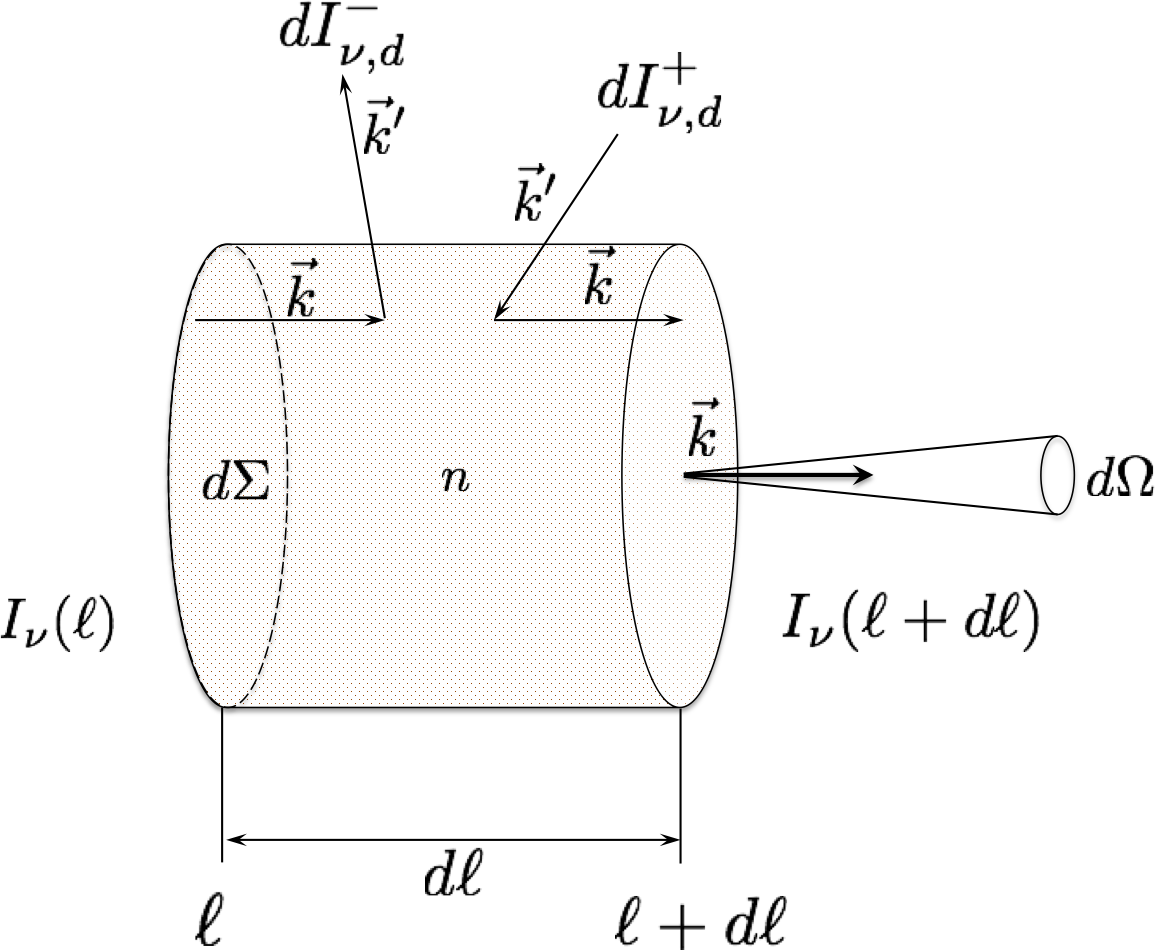
\includegraphics[width=0.5\columnwidth]{Transfert.png}
\caption{Layout of the inifinitesimal volume defined in Sec.~\ref{sec:optdep} and the relevant quantities in the balance of $E_\nu$.}
\label{fig:transfer}
\end{center}
\end{figure}

Consider an infinitesimal volume of surface area $d\Sigma$ and depth $d\ell$ which has a constant density $n$ of scattering and absorbing particles, illustrated on Fig.~\ref{fig:transfer}. To balance the spectral energy $dE_\nu (\ell)$ and $dE_\nu (\ell + d\ell)$ in and out of the volume, one must consider source terms that produce or drain spectral energy in the infinitesimal volume and exchange terms that produce or drain spectral energy on the interface $d\Sigma$: \\
\begin{equation}
d E_\nu (\ell + d\ell) - d E_\nu (\ell) = d^2 E_\nu^{\mathrm{sources}} + d I_\nu^{\mathrm{exchanges}} dt
\end{equation} \\ The volumic source terms consist of emissions and absorptions, $d^2 E_\nu^{\mathrm{sources}} = d^2 E_{\nu, e} + d^2 E_{\nu, a}$, and define the emissivity $\epsilon_\nu$ of the medium and the absorption opacity $\kappa_{\nu, a}$ such that \\
\begin{equation}
\left\{
\begin{array}{l}
d^2 E_{\nu, e} = \epsilon_\nu ~dV dt d\Omega d\nu\\
d^2 E_{\nu, a} = - \kappa_{\nu, a} d\ell dE_\nu (\ell)
\end{array}
\right.
\end{equation} \\ Exchanges with the exterior include scattering photons into and out of the infinitesimal volume:
\begin{equation}
d I_\nu^{\mathrm{exchanges}} = d I_{\nu, d}^{+} + d I_{\nu, d}^{-} 
\end{equation} which defines the diffusion coefficient $\sigma_\nu$:
\begin{equation}
d I_{\nu, d}^{\pm} = \pm \sigma_\nu I_\nu d\ell = \pm S_{\nu, d} n d\ell I_\nu
\end{equation} \\

When the source light interacts with the foreground, the tranfer equation can thus be expressed as \\
\begin{equation}
\frac{d I_\nu}{d \tau_\nu} = S_\nu - I_\nu
\end{equation} \\ where $S_\nu$ is the ``source function'', the ratio between all gain terms, \textit{i.e.} the emissivity of the medium and photons scattering into it, and all drain terms which include the medium's opacity and the photons scattering out : \\
\begin{equation}
S_\nu (I_\nu) = \cfrac{\epsilon_\nu + \sigma_\nu J_\nu}{\kappa_\nu + \sigma_\nu}
\end{equation} \\ The terms in the denominator define the medium's absorption + diffusion opacity $d\tau_\nu$, \textit{a.k.a.} the \textbf{optical depth} \\
\begin{empheq}[box=\mymath]{equation}
d\tau_\nu = (\kappa_\nu + \sigma_\nu) d\ell
\end{empheq} \\ When integrating along the light's path, a photon of frequency $\nu$ has a survival probability\footnote{meaning a probability of not being scattered or absorbed} proportional to $1 - e^{- \tau_\nu}$. A short optical depth with respect to the medium's characteristic length means the medium is opaque at that frequency. When the optical depth is of the order of the medium's characteristic length scale, it is considered transparent for that frequency. CMB photons, which have free streamed from their last scattering at some $z \simeq 1,050$ traverse the IGM, which is transparent for all the frequency range from their initial optical (yellow) to their current microwaves. As the first stars, AGNs or some other sources heat up the IGM, it becomes ionized again at some yet poorly constrained redshift $7 \lesssim z_\star \lesssim 20$, which corresponds to when $50\%$ the neutral Hydrogen is ionised. From then to now, the CMB photons can again Coulomb-scatter off the free electrons, which smear the temperature fluctuations. The analysis of the temperature power spectrum of the Planck collaboration~\citep{Planck2015} yields a value for this optical depth to reionization of \\
\begin{equation}
\tau_\star = 0.066 \pm 0.016
\end{equation} \\ corresponding to a reionization redshift of \\
\begin{equation}
z_\star = 8.8^{+1.7}_{-1.4}
\end{equation} \\

\subsubsection{The Lyman-Alpha Absorption}

The Lyman series of Hydrogen correspond to the set of UV emission lines due to the electron transitioning from an excited state $n \geqslant 2$ to the ground state $n=1$, with $n$ the principal quantum number. The Lyman-alpha (Ly-$\alpha$) and Lyman-beta (Ly-$\beta$) are the first and second transitions of the Lyman series, from the ground $n=1$ to the $n=2$ (respectively $n=3$) states. The energy of the Lyman series of transitions is determined by the Rydberg formula
\begin{equation}
\label{eq:Rydberg}
\frac{h c}{\lambda} = R_{\mathrm{H}} \times  \left( 1 - \frac{1}{n^2} \right)
\end{equation} where the Rydberg constant $R_\mathrm{H} = 13.6~\mathrm{eV}$ in units of $hc$. The Ly-$\alpha$ $(n = 2 ~\mapsto~ n=1)$ and Ly-$\beta$ $(n = 3 ~\mapsto~ n=1)$ transitions thus have UV wavelengths of $\lambda_\alpha = 121.6~\mathrm{nm}$ and $\lambda_\beta = 102.6~\mathrm{nm}$ respectively. The Ly-$\alpha$ $\lambda 1216$ and Ly-$\beta$ $\lambda 1026$ emission lines are easily recognisable in the spectra of quasars. When a photon from the background quasar interacts with the neutral Hydrogen in the IGM, the electron can, inversely, be excited from its ground state to the $n=2$ and $n=3$ quantum states, known as the Ly-$\alpha$ and Ly-$\beta$ \emph{absorption} respectively. The incoming photon has energy $E_\gamma \left( 1 - v_\parallel / c \right)$ in the reference frame of the neutral Hydrogen atom of velocity $\vec{v} = \vec{v}_\parallel + \vec{v}_\perp$ (radial and normal to the photon's incoming direction). The probability of being absorbed to $n=1 \mapsto n=2$ is $e^{-\tau}$ with the Ly-$\alpha$ optical depth given by the Beert-Lambert law

\begin{equation}
\label{eq:beertlambert}
d\tau = n_{\mathrm{\textsc{Hi}}} ~\sigma_{\mathrm{Ly}\alpha} ~dr \times  \left\{
\begin{array}{ll}
1 & \text{if}~E_\gamma \left( 1 - \frac{v_\parallel (r)}{c} \right) = E_{\mathrm{Ly}\alpha} \\
0 & \text{else}
\end{array}
\right.
\end{equation} where $\sigma_{\mathrm{Ly}\alpha}$ is the Ly-$\alpha$ transition's cross section and $E_{\mathrm{Ly}\alpha} = 1.02~\mathrm{keV}$ its rest energy (Eq.~\ref{eq:Rydberg}). The radial physical distance is 
\begin{equation}
\label{eq:drdzbl}
dr = \frac{dz}{1+z}~\frac{c}{H_0 \times \sqrt{\Omega_m (1+z)^3 + 1 - \Omega_m}}
\end{equation} Since we probe density fluctuations in the Hubble flow, quantities are measured in velocity space along the line-of-sight. In velocity space, the Ly-$\alpha$ optical depth
\begin{equation}
	\tau \left(v\right) = \int_{0}^{v} \mathrm{d}v'_{\parallel} ~ \frac{n_{\rm{H_I}} \sigma_{\rm{Ly}\alpha}\left(z\right)}{\nabla v'_{\parallel}}
		\label{eq:tau}
\end{equation} is actually sensitive to the velocity gradient parallel to the line-of-sight, $\nabla v_{\parallel}$, and not the absolute value of the velocity. \\

Neutral Hydrogen in the intergalactic medium (IGM) is present wherever photo-ionization by the ultraviolet (UV) background is balanced by electron recombination $\gamma + \rm{H} \rightleftharpoons e^{-} + \rm{H}^{+}$. The density of neutral Hydrogen (\textsc{Hi}) can thus be obtained by equating the interaction rates of both reactions and by setting global neutrality ($n_e = n_p$):
\begin{equation}
	n_{\mathrm{\textsc{Hi}}} = \left( \frac{\sigma_{\mathrm{comb}} \sqrt{2 k_b/m_e}}{c ~\sigma_{\rm{ion}}} \right) \frac{n_b^2 T^{-0.7}}{n_{\gamma_{\rm{UV}}}}
		\label{eq:Hydrogen}
\end{equation} where $\sigma_{\rm{comb, ion}}$ are respectively the recombination and photo-ionization cross-sections and $n_{b, \gamma_{\rm{UV}}}$ the baryon and Ultra Violet (UV) photon densities. \\


%%%%%%%%%%%%%%%%%%%%%%%%%%%%%%%%%%%
\subsection{The Lyman-Alpha Forest}
%%%%%%%%%%%%%%%%%%%%%%%%%%%%%%%%%%%


\subsubsection{Definition}
\label{sec:def_lya}

With light from a distant quasar serving as a background source, their spectra encode the Ly-$\alpha$ optical depth (Eq.~\ref{eq:tau}). The QSO's observed and intrinsic flux at the $\lambda = (1+z) \times 1216$ {\AA} observed wavelength is
\begin{equation}
	\varphi_{\rm{obs}} \left(\lambda\right) = e^{- \tau} ~\varphi_{\rm{qso}} \left(\lambda\right)
		\label{eq:flux}
\end{equation} Because of cosmological redshift, the rest-frame wavelength of the Ly-$\alpha$ absorption gets redshifted from its observed wavelength as the quasar signal travels to Earth in an expanding Universe. Hence a series of absorption features  between the Ly-$\alpha$ $\lambda 1216$ and Ly-$\beta$ $\lambda 1026$ emission lines in the spectra of high-redshift QSOs that entails the distribution of neutral Hydrogen along the line-of-sight. This so-called \textbf{Ly-}$\pmb{\alpha}$ \textbf{forest} is a widely-used tool to probe density fluctuations at intergalactic scales. It is the blue region highlighted in Fig.~\ref{fig:boss_spectrum}. Ly-$\alpha$ absorption can still occur redwards of the Ly-$\beta$ emission line. However, it becomes intermingled with the Ly-$\beta$ absorption's own forest. Disentangling them would require studying their cross-correlation. \\

To avoid contaminating the power spectrum with astrophysical effects in the vicinity of the Ly-$\alpha$ and Ly-$\beta$ emission lines, we define our working Ly-$\alpha$ forest region as the range of the QSO's rest-frame wavelengths 
\begin{equation}
1,040~\leqslant ~ \frac{\lambda_0}{\mathrm{\AA}} ~\leqslant ~1,200
\end{equation} \textit{i.e.} some $\sim 4 \times 10^3~\mathrm{km}~s^{-1}$ away from these emission line peaks. Typically, a $z_{\mathrm{qso}} = 4$ quasar has a Ly-$\alpha$ forest that spans $\Delta z \simeq 0.65$. To improve the redshift resolution to $\Delta z < 0.2$, the Ly-$\alpha$ forest is split into three consecutive non-overlapping equi-length sectors. This ensures that each of these $z$-sector lies in one of the spectroscopic arms of the instrument as well as to avoid parts of the forest that contains Damped Ly-$\alpha$ or Lyman Limit systems. \\

\subsubsection{The Transmitted Flux Power Spectrum}

Perhaps the most conveniant and widely-used statistical tool to compare observations with theoretical predictions is the one-dimensional flux power spectrum~\citep{Croft1999}. It is obtained by the Fourier transform of the QSO's transmitted flux fraction
\begin{equation}
	\delta_\varphi (\lambda) = \frac{\varphi (\lambda) - \langle x_\varphi \rangle}{\langle x_\varphi \rangle} = \frac{e^{-\tau}}{e^{-\tau_{\rm{eff}}}} - 1
		\label{eq:delta_flux}
\end{equation} normalized by a mean transmitted flux fraction $x_\varphi = \varphi_{\mathrm{obsserved}} / \varphi_{\mathrm{emitted}}$ which defines an effective optical depth $\langle x_\varphi \rangle = e^{- \tau_{\rm{eff}}}$. \\

The flux power spectrum in the Ly-$\alpha$ forest is obtained by deconvolving the power spectrum of the transmitted flux fraction defined in Eq.~\ref{eq:delta_flux} from the instrumental window function $W$ after substracting the (white) noise power spectrum, and averaging over the entire set of Ly-$\alpha$ forest:
\begin{empheq}[box=\mymath]{equation}
	P_{\rm{Ly}\alpha} (k) = \left\langle \frac{\vert \tilde{\delta_\varphi}(k) \vert^2 - P_{\rm{noise}}(k)}{W^2 (k)} \right\rangle_{QSOs}
		\label{eq:PLya_def}
\end{empheq} 



\subsubsection{Measuring the Power Spectrum in Quasar Spectra}

From each of the quasar spectra samples I describe in Sec.~\ref{sec:pfdata}, only the Ly-$\alpha$ forests with a high signal-to-noise ratio, no broad absorption lines, damped Ly-$\alpha$ or Lyman Limit systems, and sufficient resolution are selected. Sky lines significantly increase the pixel noise in the data. Once identified using a method detailed in \cite{Lee2013}, the pixels which cover $\lambda = 5577, 5890, 6300, 6364$ and $6864$ {\AA} are masked and replaced by the flux averaged over the rest of the unmasked forest. For the medium-resolution quasar spectra from XSHOOTER described in Sec.~\ref{sec:mrs}, this bias is negligeable due to the low number of sky lines in this wavelength region coupled with the resolution of the spectrograph. For the lower resolution spectra fro BOSS described in Sec.~\ref{sec:lrs}, the bias can reach $15\%$ (at most) at the small $k$ for the $3.5 < \langle z \rangle \leq 3.7$ redshift bin containing the strongest sky emission line, \textsc{Oi} $\lambda5577$. This bias is corrected for in a procedure described in \cite{Palanque-Delabrouille2013}. \\

\begin{figure}
\begin{center}
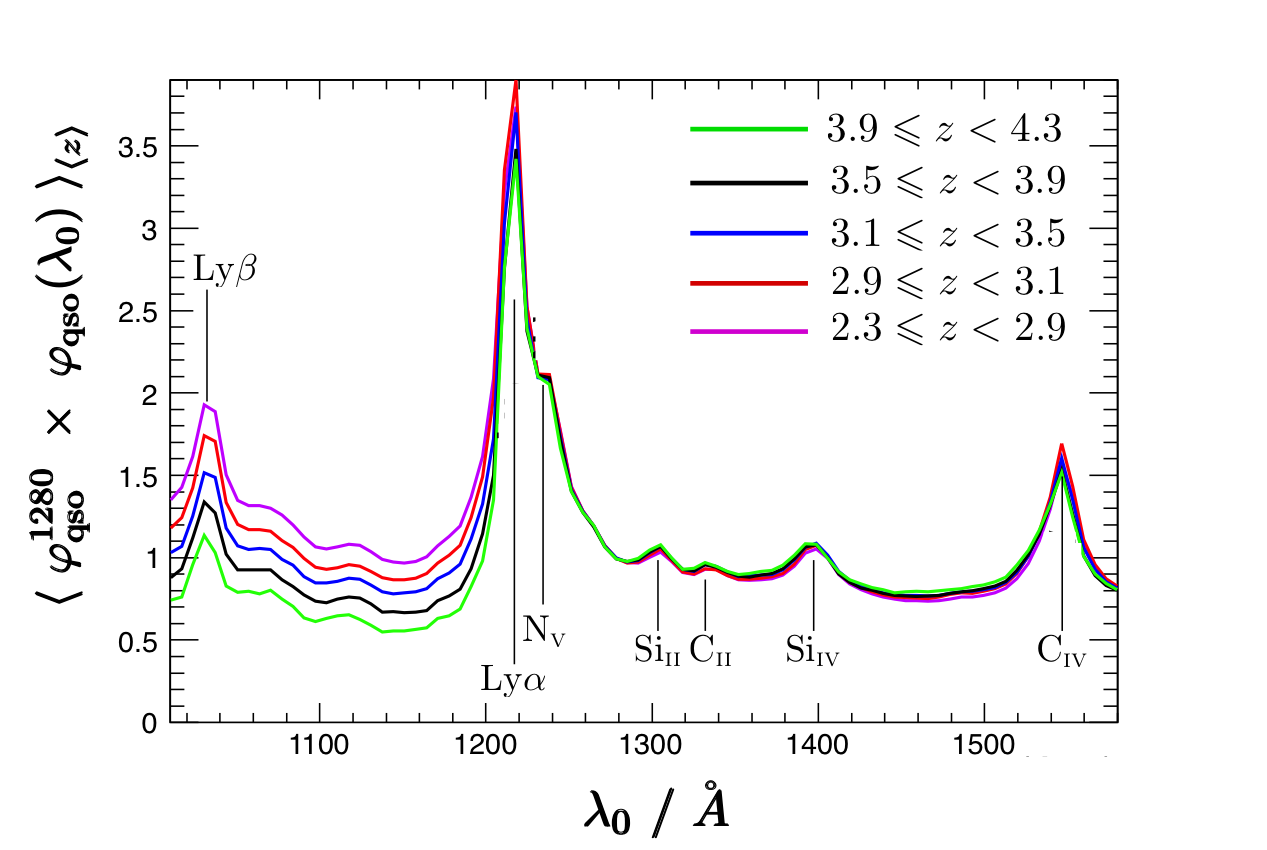
\includegraphics[width=0.5\textwidth]{SDSS/qso_stack_boss.png}~%
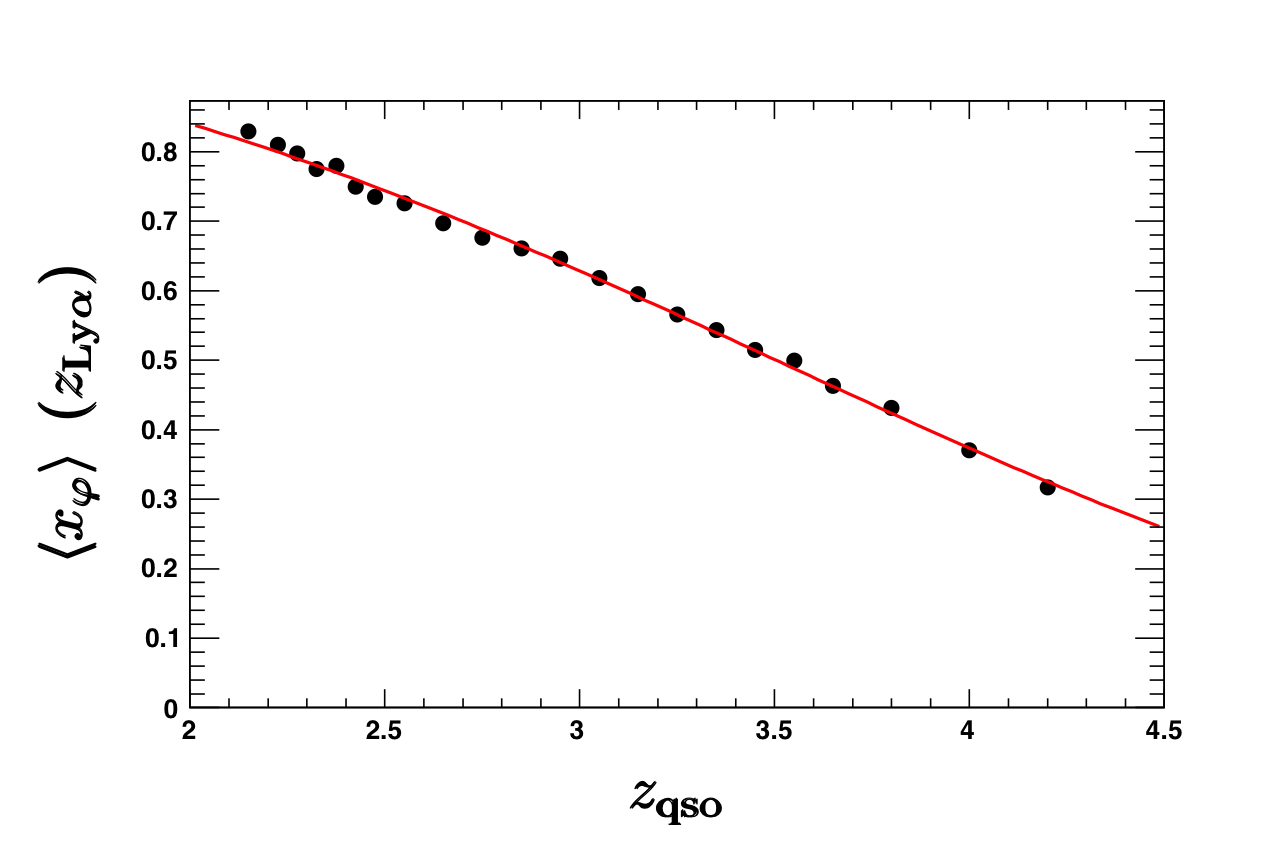
\includegraphics[width=0.5\textwidth]{SDSS/LUT2.png}
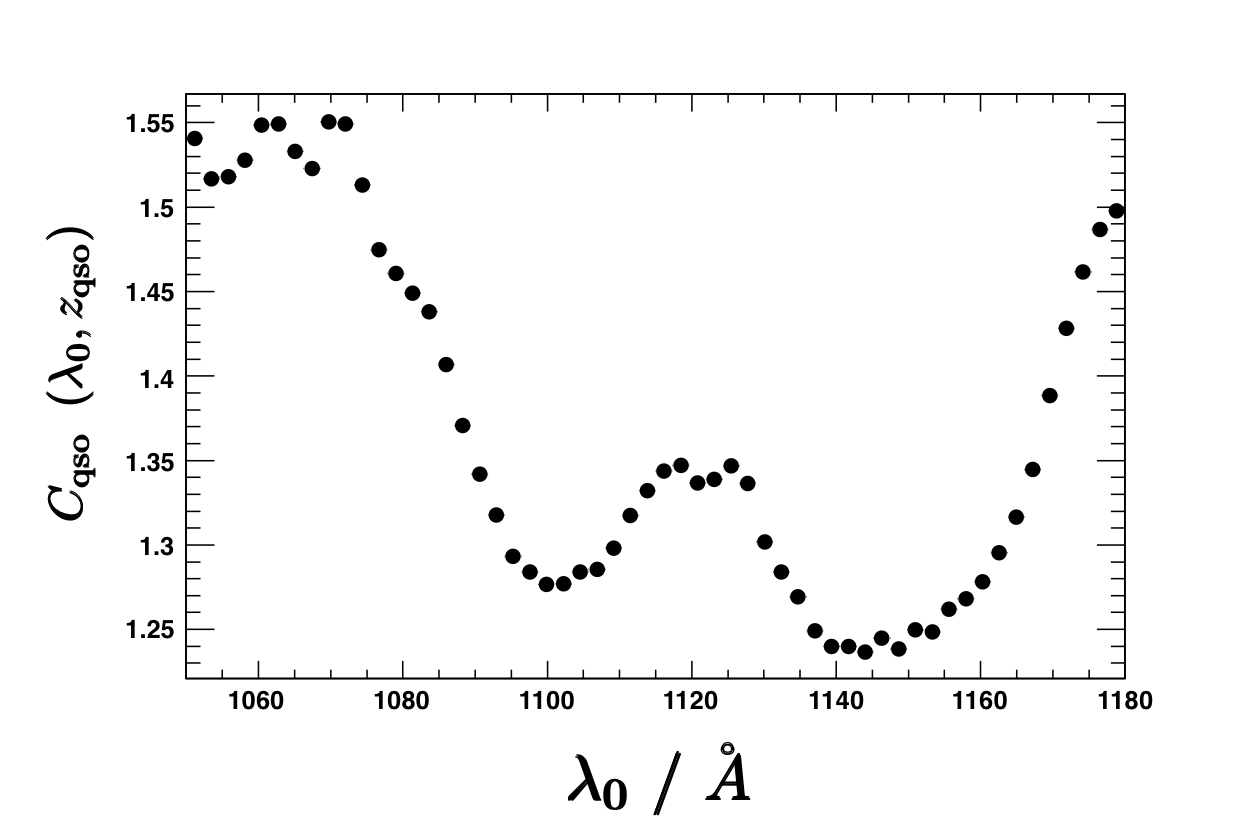
\includegraphics[width=0.5\textwidth]{SDSS/LUT1.png}~%
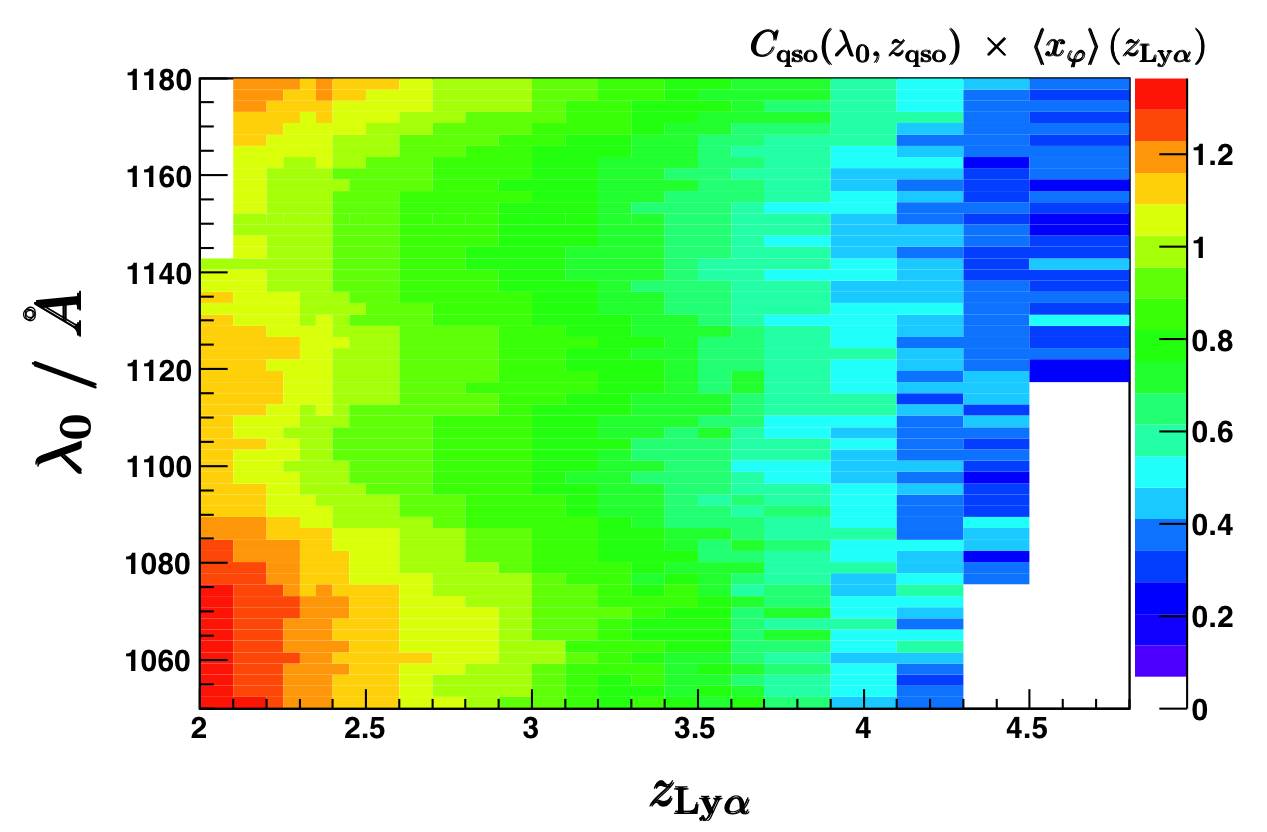
\includegraphics[width=0.5\textwidth]{SDSS/LUT3.png}
\caption{\textbf{Top Left:} Observed BOSS quasar spectra in their rest frame wavelength, normalised to the $1280$ {\AA} pixel in five different redshift bins. \textbf{Top Right:} Mean transmitted flux fraction as a function of redshift. \textbf{Bottom Left:} Quasar mean absorption in the Ly-$\alpha$ forest. \textbf{Bottom Right:} Quasar continuum times the mean transmitted flux fraction.}
\label{fig:LUT}
\end{center}
\end{figure}

The transmitted flux fraction in Eq.~\ref{eq:delta_flux} is then computed by stacking the selection of Ly-$\alpha$ forests in their rest-frame using $\lambda_0 = \lambda / (1 + z_\mathrm{qso})$. To do so requires normalizing the unabsorbed\footnote{outside of the Ly-$\alpha$ forest range, \textit{i.e.} red-wards of the Ly-$\alpha$ emission line} flux $C_\mathrm{qso}~(\lambda, z_\mathrm{qso})$, \textit{a.k.a.} the QSO's continuum plotted in the lower left panel of Fig.~\ref{fig:LUT}, by the value of the flux at $\varphi (\lambda_0 = 1280 \pm 10$ {\AA}$)~\doteq ~\varphi_{\mathrm{qso}}^{1280}$ to average out the fluctuating Ly-$\alpha$ absorption. Sky-line-affected pixels are not included when computing this normalisation. Since  the mean quasar continuum is flat in the normalizing region, this rejection of a few pixels does not bias the mean pixel value. The upper left panel of Fig.~\ref{fig:LUT} displays the normalized flux in 5 redshift bins. Broad quasar emission lines are clearly visible, such as (from blue to red): Ly-$\beta~\lambda 1026$, Ly-$\alpha~\lambda 1216$, N\textsc{v}~$\lambda 1240$, Si\textsc{ii}~$\lambda 1309$, the C\textsc{ii}~$\lambda 1335~\lambda 1336$ doublet, Si\textsc{iv}~$\lambda 1400$, and C\textsc{iv}~$\lambda 1549$. There are more \textsc{Hi} absorbers along the QSO line-of-sight, which appear blue-wards of the quasar's Ly-$\alpha$ emission peak, at higher redshifts since the Universe's scale factor is smaller and the IGM has a lower ionized fraction. This translates into less transmitted flux at the higher redshift bins (black and green lines). The quantity $\varphi (\lambda) / (~\varphi_{\mathrm{qso}}^{1280} \times  C_\mathrm{qso}(\lambda) ~)$ corresponds to the transmitted flux fraction. \\

The \emph{normalized} flux fraction defined in Eq.~\ref{eq:delta_flux} is normalized with respect to the mean transmitted flux fraction at the \textsc{Hi} absorber redshift $\langle x_\varphi \rangle~(z_{\mathrm{Ly}\alpha})$, featured in the upper right panel of Fig.~\ref{fig:LUT}. Its redshift dependance approximates a power law
\begin{equation}
\langle x_\varphi \rangle (z_{\mathrm{Ly}\alpha}) \propto e^{- \tau_{\mathrm{eff}}} \propto e^{A_\tau (1+z_{\mathrm{Ly}\alpha})^{\eta_\tau}} 
\end{equation} whose fit $A_\tau \simeq 4.6 \times 10^{-3}$ and $\eta_\tau \simeq 3.3$ is in agreement with measurements of the effective optical depth $\tau_\mathrm{eff}$ in \cite{Meiksin2009, Becker2011}. For a pixel of wavelength $\lambda$, the corresponding \textsc{Hi} absorber redshift is infered from $z_{\mathrm{Ly}\alpha} = \lambda / \lambda_{\mathrm{Ly}\alpha} + 1$ where $\lambda_{\mathrm{Ly}\alpha} = 1215.67$ {\AA}. The product $C_\mathrm{qso}(\lambda, z_{\mathrm{qso}}) \times \langle x_\varphi \rangle (z_{\mathrm{Ly}\alpha})$ is assumed to be universal for all quasars at $z_\mathrm{qso}$ and is illustrated in the bottom right panel of Fig.~\ref{fig:LUT}. The normalized flux fraction is thus \\
\begin{empheq}[box=\mymath]{equation}
\delta_\varphi (\lambda) = \frac{\varphi (\lambda)}{\langle \varphi \rangle} - 1 = \frac{\varphi (\lambda)}{\varphi_{\mathrm{qso}}^{1280}} \times \frac{1}{C_{\mathrm{qso}} (\lambda, z_\mathrm{qso}) \times \langle x_\varphi \rangle (z_{\mathrm{Ly}\alpha})} - 1
\end{empheq} \\ where the quantity $\varphi_{\mathrm{qso}}^{1280} \times C_{\mathrm{qso}} (\lambda, z_\mathrm{qso}) \times \langle x_\varphi \rangle (z_{\mathrm{Ly}\alpha})$ represents the mean expected flux. 

\subsubsection{Uses in Cosmology}

From Eq.~\ref{eq:Hydrogen}, the neutral Hydrogen density is an explicit function of the baryon density $n_b$ and the intergalactic gas temperature. As such, the Ly-$\alpha$ forest is of great interest for cosmology because it entails information on the neutral Hydrogen content of the IGM. Analytical models \citep{Bi1993, Miralda-Escude1993, Hui1997} as well as hydrodynamics simulation \citep{Cen1994a, Zhang1995, Hernquist1996,
Croft1997} showed that the optical depth is proportional to the Hydrogen density, itself a tracer of the baryon density through $n_{\textsc{Hi}} = A \rho_b^\eta$ with $\eta \sim 1.5-2.0$. The transmitted flux fraction can thus be written
\begin{equation}
x_\varphi = \frac{\varphi_{\mathrm{obs}}}{\varphi_{\mathrm{qso}}} = e^{- \tau} = e^{-A\rho_b^\eta}
\end{equation} However, because this coupling is non-linear and the fact that $A$ is poorly known, it is usually impossible to evaluate the baryon density. \\

The cross section of the Ly-$\alpha$ transition is very high and the fact that the absorption is not completely saturated comes
from the high ionisation fraction of the IGM, as shown in \cite{Gunn1965}. This ionisation comes from the UV photon flux generated
by star forming galaxies and active galactic nuclei and thus depends on the redshift. Moreover, the Universe expansion induces a
diminution of the hydrogen mean density with time, proportional to $(1+z)^3$. These two dependencies make the Ly-$\alpha$ forest bias dependent on the redshift. \\

Consequently, \cite{Croft1998} have suggested a technique for recovering the initial power spectrum of density fluctuations
directly from the fluctuations of the optical depth measured from Ly-$\alpha$ forest spectra. One can use the Ly-$\alpha$
forest to constrain cosmological parameters, from Eqs.~\ref{eq:beertlambert}, and~\ref{eq:drdzbl}. On the one
hand, one must use QSO spectra to obtain the power spectrum of the transmitted flux in the Ly-$\alpha$ forest and recover the power
spectrum of density fluctuation. On the other hand, numerical simulations with different input parameters must be run to extract
the power spectrum of mass density fluctuations. Then one can compare the measured power spectrum with the simulated ones,
inferring the best set of input parameters to reproduce the observations. \\

\begin{figure}
\begin{center}
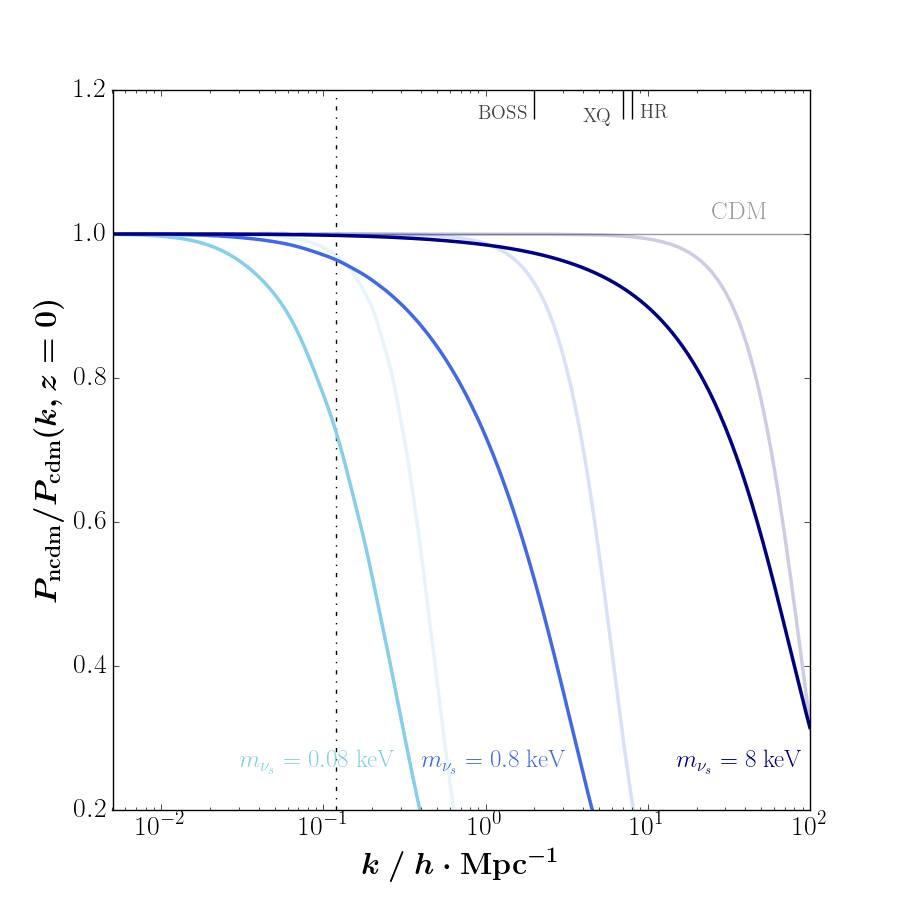
\includegraphics[width=0.5\columnwidth]{WDM_T1D.png}~%
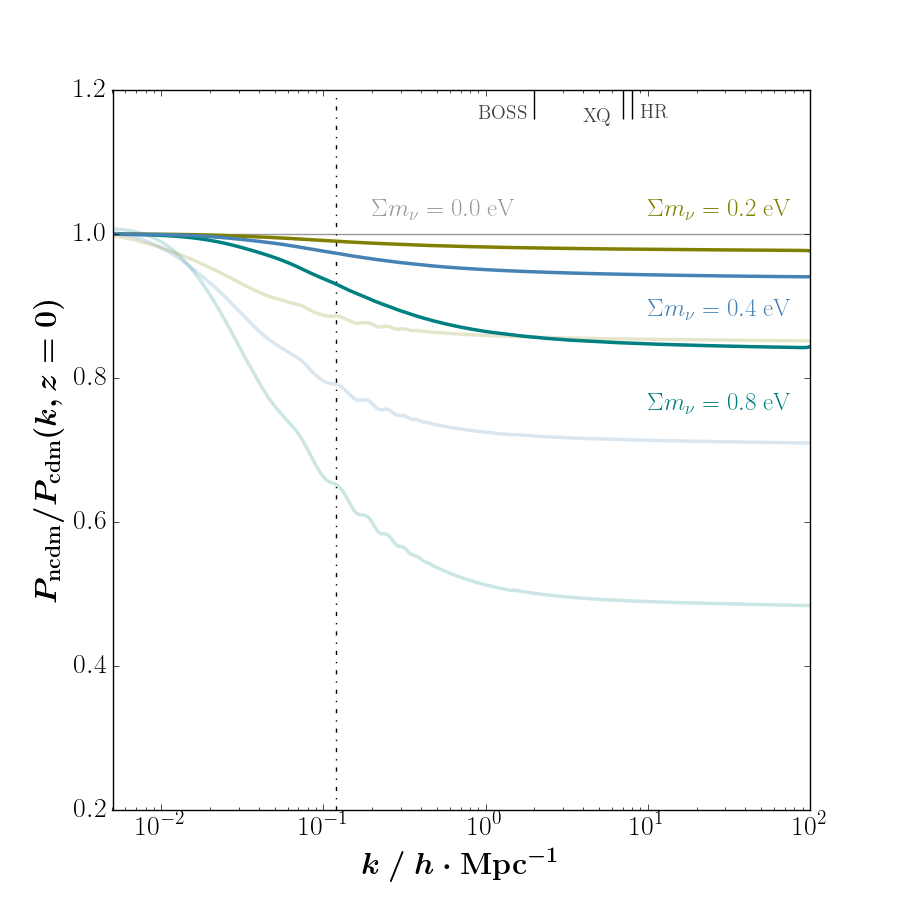
\includegraphics[width=0.5\columnwidth]{CHDM_T1D.png}
\caption{One-dimensional matter power spectrum at $z=0$ in NCDM cosmologies normalized to that of the benchmark CDM model. The 3D matter power spectrum ratio are superimposed as the semi-transparent curves for comparative purposes. The `BOSS', `XQ', and `HR' ticks correspond to the highest $k$ probed by the 3 types of Ly-$\alpha$ forest data set I use in Sec.~\ref{sec:pfdata} and Sec.~\ref{sec:data}. \textbf{Left:} pure WDM for $m_{\nu_s} = 8 \times 10^{-2, -1, 0}~\mathrm{keV}$. \textbf{Right:} mixed C+HDM with $\sum m_\nu = 0.2, 0.4, 0.8~\mathrm{eV}$.}
\label{fig:t1d}
\end{center}
\end{figure}

Since neutral Hydrogen in the IGM is a (biased) tracer for the (total) matter density fluctuations, Ly-$\alpha$ forests can serve to probe the $10^{1-2}~ h^{-1}\mathrm{Mpc}$ scales at which neutrino free-stream. The flux power spectrum is computed along a line-of-sight, and as such the Ly-$\alpha$ forest power spectrum (when averaging over an entire set of Ly-$\alpha$ forests) is uni-dimensional. In Fig.~\ref{fig:t1d}, I feature the linear matter 1D power spectrum computed in the linear regime, which is obtained from the 3D power spectrum \\

\begin{empheq}[box=\mymath]{equation}
\label{eq:1dps}
P^{\mathrm{1d}}_m (k_\parallel, z) ~\doteq~ \int \frac{d\vec{k}_\perp}{(2 \pi)^2}~P^{\mathrm{3d}}_m (k_\parallel, \vec{k}_\perp, z)
 ~=~ \int_{k_\parallel}^{\infty} \frac{dk}{2 \pi} ~k~P^{\mathrm{3d}}_m (k, z)
\end{empheq} \\ I overlay the 3D power spectra which I computed in Chap.~\ref{chap:structure}. The vertical dotted line is the lowest $k$ scale probed by the Ly-$\alpha$ forest power spectrum. In the 1D case, the highest $k$ value probed by the different quasar samples I describe in Sec.~\ref{sec:pfdata}. The 1D power spectra of the $\sum m_\nu = 0.2, 0.4$ and $0.8~\mathrm{eV}$ are significantly closer to the 1D power spectrum of CDM. Measuring $\sum m_\nu = 0.2~\mathrm{eV}$ neutrino masses with Ly-$\alpha$ forests requires a precision of about a percent. In Chap.~\ref{chap:Simulations}, I construct the Ly-$\alpha$ power spectrum for these NCDM models, which require solving the hydrodynamics in the non-linear regime.


\clearpage
